\section{Case Study: Huffman Coding}

\subsection{Formal Problem Statement}
Let A be defined as the set of alphabets. ( $A = \{ a_0, a_1, a_2, ..., a_n \}$ )\\
Let W be defined as the set of weights for which $w_i = \text{Weight}(a_i)$.  ($W = \{ w_0, w_1, w_2, ..., w_n \}$)
Let C be defined as the set of (binary) codewords for which $c_i = \text{CodeWord}(a_i)$.\\\\
Assume there exists $n$ alphabets, each with a weight $w_i$. Find and define the codewords $c_i$ for each respective alphabet $a_i$ such that $\sum\limits_{i=0}^{n} w_i \cdot length(c_i)$ is the smallest possible.

\subsection{Informal Problem Statement}
Given a set of symbols and their weights (probabilities), find a prefix-free binary code with minimum expected codeword length.

\subsection{Greedy Choice}
Choose the two alphabets with the lowest weight. 

\subsection{Steps}
\begin{enumerate}
	\item Pick two letters $x$ and $y$ from the alphabet A with the lowest frequencies or weight $w_i$.
	\item Create a subtree with $x$ and $y$ as leaves. We will define the root as $z$.
	\item The frequency or weight of node $z$ will be define as $w_z = w_x + w_y$.
	\item Remove $x$ and $y$ from alphabet.\\
		$ A^\prime = A - \{ x, y \}$
	\item Insert $z$ into the alphabet.\\
		$ A^\prime = A + \{ z \} $
	\item Repeat this process until the set of alphabets $A$ consists of only one alphabet.
\end{enumerate}

\newpage

\subsection{Example}
\textbf{Let $A = \{ a, b, c, d, e \}$ and $W = \{ 30, 16, 6, 15, 35 \}$. Find their corresponding Huffman codes.}

\subsubsection*{Merge $c$ and $d$}
\begin{minipage}{0.35\linewidth}
	\flushleft
	\begin{tabular}{| c | c |}
		\hline
		Alphabet	&	Weight\\
		\hline
		e			&	35\\
		\hline
		a			&	30\\
		\hline
		b			&	16\\
		\hline
		d			&	15\\
		\hline
		c			&	6\\
		\hline
	\end{tabular}
\end{minipage}
\qquad
\begin{minipage}{0.65\linewidth}
	\centering
	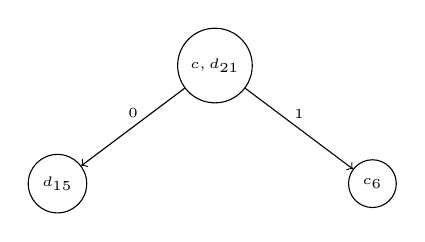
\begin{tikzpicture}[level/.style={sibling distance=40mm/#1}]
	\node [circle,draw] {\tiny$c,d_{21}$}
	child {
		node [circle,draw] {\tiny$d_{15}$}
		edge from parent [->] node [above] {\tiny 0}
	}
	child {
		node [circle,draw] {\tiny$c_6 $}
		edge from parent [->] node [above] {\tiny 1}
	};
	\end{tikzpicture}
\end{minipage}


\subsubsection*{Merge $c,d$ and $b$}
	\begin{minipage}{0.35\linewidth}
		\flushleft
		\begin{tabular}{| c | c |}
			\hline
			Alphabet	&	Weight\\
			\hline
			e			&	35\\
			\hline
			a			&	30\\
			\hline
			c,d			&	21\\
			\hline
			b			&	16\\
			\hline
		\end{tabular}
	\end{minipage}
	\qquad
\begin{minipage}{0.65\linewidth}
	\centering
	\begin{tikzpicture}[level/.style={sibling distance=60mm/#1}]
	\node [circle,draw] {\tiny$b,c,d_{37}$}
	child {
		node [circle,draw] {\tiny$c,d_{21}$}
		child {
			node [circle,draw] {\tiny$d_{15}$}
			edge from parent [->] node [above] {\tiny 0}
		}
		child {
			node [circle, draw] {\tiny$c_{6}$}
			edge from parent [->] node [above] {\tiny 1}
		}
		edge from parent [->] node [above] {\tiny 0}
	}
	child {
		node [circle,draw] {\tiny$b_{16} $}
		edge from parent [->] node [above] {\tiny 1}
	};
	\end{tikzpicture}
\end{minipage}

\subsubsection*{Merge $e$ and $a$}
\begin{minipage}{0.35\linewidth}
\flushleft
	\begin{tabular}{| c | c |}
		\hline
		Alphabet	&	Weight\\
		\hline
		b,c,d			&	37\\
		\hline
		e			&	35\\
		\hline
		a			&	30\\
		\hline
	\end{tabular}
\end{minipage}
\qquad
\begin{minipage}{0.30\linewidth}
	\centering
	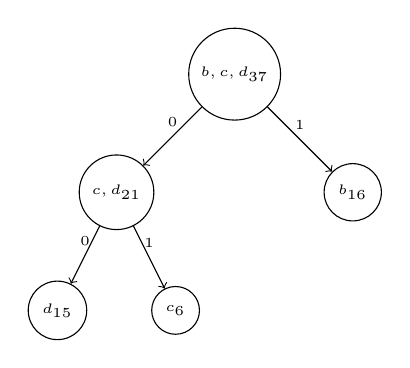
\begin{tikzpicture}[level/.style={sibling distance=30mm/#1}]
	\node [circle,draw] {\tiny$b,c,d_{37}$}
	child {
		node [circle,draw] {\tiny$c,d_{21}$}
		child {
			node [circle,draw] {\tiny$d_{15}$}
			edge from parent [->] node [above] {\tiny 0}
		}
		child {
			node [circle, draw] {\tiny$c_{6}$}
			edge from parent [->] node [above] {\tiny 1}
		}
		edge from parent [->] node [above] {\tiny 0}
	}
	child {
		node [circle,draw] {\tiny$b_{16} $}
		edge from parent [->] node [above] {\tiny 1}
	};
	\end{tikzpicture}
\end{minipage}
\begin{minipage}{0.30\linewidth}
	\centering
	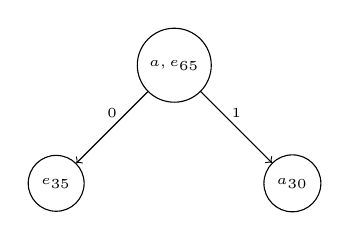
\begin{tikzpicture}[level/.style={sibling distance=30mm/#1}]
	\node [circle,draw] {\tiny$a,e_{65}$}
	child {
		node [circle,draw] {\tiny$e_{35}$}
		edge from parent [->] node [above] {\tiny 0}
	}
	child {
		node [circle,draw] {\tiny$a_{30} $}
		edge from parent [->] node [above] {\tiny 1}
	};
	\end{tikzpicture}
\end{minipage}


\subsubsection*{Merge $a,b,c,d$ and $e$}
\begin{minipage}{0.35\linewidth}
	\flushleft
	\begin{tabular}{| c | c |}
		\hline
		Alphabet	&	Weight\\
		\hline
		a,e			&	65\\
		\hline
		b,c,d		&	37\\
		\hline
	\end{tabular}
\end{minipage}
\qquad
\begin{minipage}{0.65\linewidth}
\centering
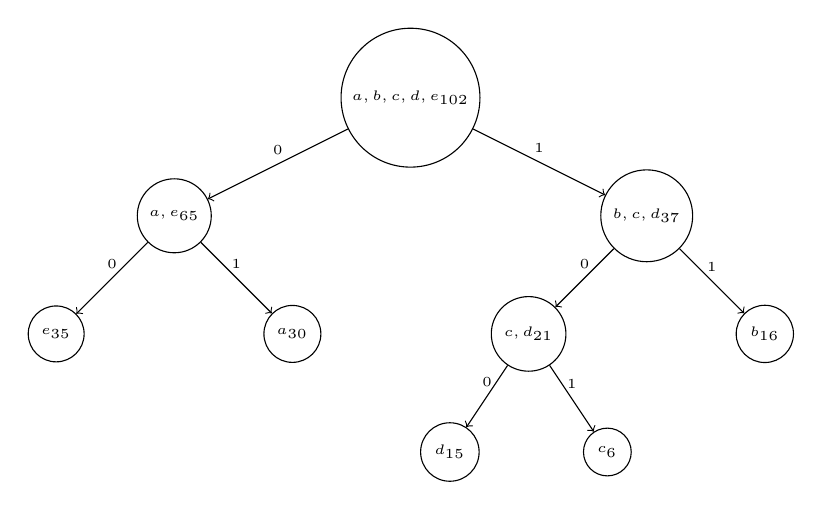
\begin{tikzpicture}[level/.style={sibling distance=60mm/#1}]
	\node [circle,draw] {\tiny$a,b,c,d,e_{102}$}
	child {
		node [circle,draw] {\tiny$a,e_{65}$}
		child {
			node [circle,draw] {\tiny$e_{35}$}
			edge from parent [->] node [above] {\tiny 0}
		}
		child {
			node [circle, draw] {\tiny$a_{30}$}
			edge from parent [->] node [above] {\tiny 1}
		}
		edge from parent [->] node [above] {\tiny 0}
	}
	child {
		node [circle,draw] {\tiny$b,c,d_{37} $}
		child {
			node [circle,draw] {\tiny $c,d_{21}$ }
			child {
				node [circle, draw] {\tiny $d_{15}$ }
				edge from parent [->] node [above] {\tiny 0}
			}
			child {
				node [circle,draw] {\tiny $c_6$}
				edge from parent [->] node [above] {\tiny 1}
			}
			edge from parent [->] node [above] {\tiny 0}
		}
		child {
			node [circle, draw] {\tiny $b_{16}$}
			edge from parent [->] node [above] {\tiny 1}
		}
		edge from parent [->] node [above] {\tiny 1}
	};
\end{tikzpicture}
\end{minipage}

\subsubsection*{Solution}

\begin{table}[H]
	\centering
	\begin{tabular}{| c | c | c |}
		\hline
		Alphabet	&	Weight	&	Codeword\\
		\hline
		e			&	35		&	00\\
		\hline
		a			&	30		&	01\\
		\hline
		b			&	16		&	11\\
		\hline
		d			&	15		&	100\\
		\hline
		e			&	6		&	101\\
		\hline
	\end{tabular}
\end{table}

